\newcommand{\realizable}{\textsc{realizable}}
\newcommand{\unrealizable}{\textsc{unrealizable}}
\newcommand{\skolems}{\textit{Skolems}}

\newcommand{\synthesisalgorithm}{
\begin{algorithm2e}[tb]
\SetAlgoSkip{}
\SetKwFor{While}{forever}{do}{}
\SetKw{KwContinue}{continue}
\KwIn{Assume-Guarantee Contract in Lustre, $(A,G)$}
\KwOut{Skolem collection \skolems, \\ \hspace{+1.3cm} Return value $\in
\{\realizable, \unrealizable\}$ of ${(A,G)}$.
\grigory{currently, it looks like the same job for realizability is performed twice. 
\aeval also does validity check (i.e., checks that the negated formula is unsat), otherwise no skolems can be generated.
I suggest to optimize it in the algorithm. Also, what is BaseCheckEngine and ExtendCheckEngine? are they simple two instances of the SMT solver?}
}
\BlankLine
$i \gets 0$;\\
$\textsc{BaseCheckEngine.SmtAdd}(\lnot BaseCheck(i))$\;
$\textsc{ExtendCheckEngine.SmtAdd}(\lnot ExtendCheck(i))$;
\\
\While{}{
	$i$++;\\
	\uIf(\label{alg:returnUnsat}){$(BaseCheckEngine.\isSat(\textsc{SmtSolve}()))$}
	{
		\Return
		\unrealizable 
	}
	$\textsc{SkolemsAdd}(\aeval(BaseCheck(i))$;\\
	\uIf(\label{alg:returnSat}){$(ExtendCheckEngine.\isUnSat(\textsc{SmtSolve}()))$}
	{
		$\textsc{SkolemsAdd}(\aeval(ExtendCheck(i)))$;\\
		\Return \skolems, \realizable
	}
}
\caption{Synthesis from Assume-Guarantee Contracts}
\label{alg:synthesis}
\end{algorithm2e}
}


\section{Synthesis from Assume-Guarantee Contracts}
\label{sec:synthesis}

%GRIGORY: no need to repeat the things since they all are mentioned in the intro (a couple of paragraphs above)
%
In this section we provide %a summary of the formal background
%that has already been established in previous work, regarding an algorithm that
%is able to generate leaf-level component implementations using only the
%information provided by the user through requirements expressed in the form of an
%Assume-Guarantee contract. Our approach supports the Linear Real
%Arithmetic (LRA) theory.
%mainly due to the limitations imposed by the underlying machinery.
% We begin with 
a brief background on Assume-Guarantee contracts, 
proceed with summarizing our earlier results on realizability
checking of contracts, and finally
present our program synthesis procedure.
%Finally, we enrich our formal definitions with an informal proof of the
%algorithm's correctness in terms of the successfully synthesized
%implementations.

\subsection{Assume-Guarantee Contracts}

In the context of requirements engineering, there have been a lot of proposed
ideas in terms of how requirements can be represented and expressed during
system design. \grigory{need for citations with examples of ``a lot'' of ideas?}
One of the most popular ways to describe these requirements is through
the notion of an Assume-Guarantee contract, where the requirements are expressed
using safety properties that are split into two separate categories. The
\emph{assumptions} of the contract correspond to properties that restrict the
set of valid inputs a system can process, while the \emph{guarantees} dictate
how the system should behave, using properties that precisely describe
the kinds of valid outputs that it may return to its environment.

\begin{figure}[t!]
	\centering
	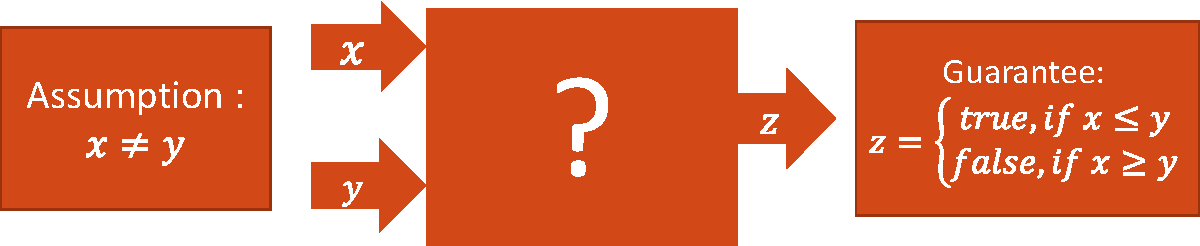
\includegraphics[width=\textwidth,height=\textheight,keepaspectratio]{real1-crop}    	
	\caption{Example of an Assume-Guarantee contract}
	\label{fg:example}
\end{figure}

As an illustrative example, consider the contract specified in
Figure~\ref{fg:example}. The component to be designed consists of two inputs,
$x$ and $y$ and one output $z$. If we restrict our example to the case of integer arithmetic,
we can see that the contract assumes that the inputs will never have the same value,
and requires that the output of the component is Boolean 
whose value depends on the comparison of the values of $x$ and $y$.
Also, notice that in the middle of the figure we depict the component using a
question mark symbol. The question mark simply expresses the fact that during
the early stages of software development, the implementation is absent or exists only partially.

Deciding existence of an implementation for the question-mark component 
that satisfies the specific contract for all possible inputs is aimed by the problem of 
\emph{realizability}, while automatically constructing a witness  of the proof 
of realizability of the contract is aimed by problem of \emph{program synthesis}.
The contract in Figure~\ref{fg:example} is obviously
\emph{realizable}, and therefore an implementation of the question-mark component exists.
Interestingly, if the assumption would be omitted then 
the contract is clearly \emph{unrealizable}, since no implementation 
is able to provide a correct output in the case where $x=y$.

\subsection{Formal Preliminaries}
\label{sec:pre}

For the purposes of this paper, we are describing a system using the types
$state$ and $inputs$. Formally, an \emph{implementation}, i.e. a
\emph{transition system} can be described using a set of initial states $I(s)$ of type $state \implies bool$, in addition to a transition relation $T(s,i,s')$ that
implements the contract and has type $state \implies inputs \implies
state \implies bool$.
 
An Assume-Guarantee contract can be formally defined by two sets, a set of
\emph{assumptions} and a set of \emph{guarantees}. The \emph{assumptions} $A$
impose constraints over the inputs, while the \emph{guarantees} $G$ are used for
the corresponding constraints over the outputs of the system and can be expressed as
two separate subsets $G_I$ and $G_T$, where $G_I$ defines the set of valid
initial states, and $G_T$ specifies the properties that need to be met during
each new transition between two states. Note that we do not necessarily expect
that a contract would be defined over all variables in the transition system,
but we do not make any distinction between internal state variables and outputs in the formalism.
This way, we can use state variables to, in some cases, simplify statements of guarantees.

\subsection{Realizability of Contracts}
The synthesis algorithm proposed in this paper is built on top of our realizability algorithm
originally presented in~\cite{Katis15:Realizability}. Using the formal foundations described in Sect.~\ref{sec:pre},
the problem of realizability is expressed using the notion of a state being \emph{extendable}:

\begin{definition}[One-step extension]
\label{def:extend}
A state $s$ is extendable after $n$ steps, denoted $\mathit{Extend}_{n}(s)$, if
any valid path of length $n-1$ starting from $s$ can be extended in response to
any input.%
%
\begin{multline*}%
\mathit{Extend}_{n}(s) \triangleq \forall i_1, s_1, \ldots, i_n, s_n.\\ A(s, i_1) \land G_T(s, i_1, s_1)
\land \cdots \land
A(s_{n-1}, i_n) \land G_T(s_{n-1}, i_n, s_n)
\implies \\
\forall i.~ A(s_n, i) \implies \exists s'.~ G_T(s_n, i, s')
\end{multline*}
\end{definition}

The algorithm for realizability uses Def.~\ref{def:extend} in two
separate checks that correspond to the two traditional cases exercised in
k-induction. For the $\mathit{BaseCheck}$, we ensure that all initial states are
extendable in terms of any path of length $k\le n$, while the inductive step of
$\mathit{ExtendCheck}$ tries to prove that all valid states are extendable.
Therefore, we attempt to find the smallest $n$, for which the two following 
$\forall\exists$-formulas are valid:%
%
\begin{equation}
\label{eq:sbcheck}
\mathit{BaseCheck}(n) \triangleq \forall k \leq n. (\forall s. G_I(s)
	  	\implies \mathit{Extend}_k(s))
\end{equation}%
%
\begin{equation}
\label{eq:echeck}
\mathit{ExtendCheck}(n) \triangleq \forall s. \mathit{Extend}_n(s)
\end{equation}

The realizability checking algorithm has been used to effectively find cases
where the traditional consistency check \grigory{what is the traditional consistency check? How does it help to the further discussion? In general, the smaller background the better.}
failed to detect conflicts between
stated requirements in case studies of different complexity and importance. It
has also been formally verified using the Coq proof assistant in terms of its
soundness, for the cases where it reports that a contract is
realizable~\cite{katis2015machine}.

\subsection{Program Synthesis from Proofs of Realizability}

\grigory{need to clearly say what is new and what is old in the section}
%While the implemented algorithm on realizability provided us with meaningful
%results during the verification of several contracts, 
The most important outcome of the work on realizability is that it 
 can be further used for solving the more complex problem of
\emph{program synthesis} i.e., to automatically
derive implementations, from the proof of the contract's
realizability.
%The limited power of SMT solvers
%in terms of solving formulas containing nested quantifiers immediately ruled
%out the prospect of using one as our primary synthesis tool. Fortunately, 
%we are able to exploit our prior results in the scope of solving validity and 
%Skolemizing $\forall\exists$-formulas (to be described in Sect.~\ref{sec:aeval}).

The idea behind our approach to solving the synthesis problem is
simple and elegant. Consider checks~\eqref{eq:sbcheck} and~\eqref{eq:echeck} that
are used in the realizability checking algorithm. Both checks require
that the reachable states explored are extendable using
Def.~\ref{def:extend}.
The key insight then is to decide if $\mathit{Extend}_{n}(s)$ is valid and generate a witness 
for each of the $n$ times that we run $\mathit{BaseCheck}$ and a final witness 
for the inductive case in $\mathit{ExtendCheck}$.

In the first order logic, witnesses for valid $\forall\exists$-formulas are represented by the Skolem functions.
Intuitively, a Skolem function expresses a connection between all universally quantified variables in the left-hand-side of the $\forall\exists$-formulas~\eqref{eq:sbcheck} and~\eqref{eq:echeck} and the existentially quantified variable $s'$ in the right-hand-side of the the formulas.
Our algorithm automatically generates such Skolem functions
while solving the validity of~\eqref{eq:sbcheck} and~\eqref{eq:echeck} and is described in details Sect.~\ref{sec:aeval}.

\synthesisalgorithm


Algorithm~\ref{alg:synthesis} provides a summary of the synthesis algorithm,
showing how it extends our previous work on realizability checking. During the
k-induction, 
\grigory{I suggest to say something like that ``Since proving validity and Skolemization are closely related tasks, we create the $\forall\exists$-formula'' for the \textit{BaseCheck(n)} and push it to the \aeval. The output is valid/invalid, and (in case of valid) also a Skolem function''.}
and for every step for which the negation of \textit{BaseCheck(n)}
is not satisfiable, we feed the corresponding $\forall\exists$-formula to
\aeval. A formula that is not satisfiable means that its negation is valid, and
as such we expect \aeval to strengthen \textit{BaseCheck(n)}'s
proof of validity. In addition to this proof, \aeval also returns a
Skolem function that essentially assigns specific values to the existentially quantified
variables, i.e. the output variables, in order to traverse into a
new state, without violating the contract. We keep repeating this process,
accumulating Skolem functions as long as the corresponding
\textit{BaseCheck(n)} is true. As soon as the inductive
step of \textit{ExtendCheck(n)} passes, we have a complete k-inductive proof
stating that the contract is realizable. We then complete our synthesis
procedure by generating a Skolem function that corresponds to the inductive
step, and return the collection of the Skolem functions to the user.



%GRIGORY: commented out the translation of A=> B => C into A /\ B => C since it is quite obvious

% Of course, 
%$\mathit{Extend}_{n}(s)$ as defined in~\eqref{def:extend} cannot
%be directly used for this purpose due to its form. This is not really an
%obstacle though, as we can rewrite the definition:
%
%\begin{multline*}
%\forall i_1, s_1, \ldots, i_n, s_n.\\ A(s, i_1) \land G_T(s, i_1, s_1)
%\land \cdots \land
%A(s_{n-1}, i_n) \land G_T(s_{n-1}, i_n, s_n)
%\implies \\
%\forall i.~ A(s_n, i) \implies \exists s'.~ G_T(s_n, i, s')
%\end{multline*}
%
%into an equivalent formula of the form $\forall \vec{x}.
%S(\vec{x}) \implies \exists \vec{y}. T(\vec{x},\vec{y})$ : 
%\begin{multline}
%	\label{ml:extendable2}
%		\forall i_1,s_1,\ldots,i_n,s_n,i. \\
%		A(s,i_1) \wedge G_T(s,i_1,s_1) \wedge \ldots \wedge
%		A(s_{n-1}, i_n) \wedge G_T(s_{n-1},i_n,s_n) \wedge A(s_n,i) \implies \\
%		\hspace{+2cm} \exists s'. G_T(s_n,i,s')
%	\end{multline}

%\begin{figure}
%\begin{small}
%\begin{verbatim}
%// for each variable in I or S,
%//   create an array of size k.
%//   then initialize initial state values
%assign_GI_witness_to_S;
%update_array_history;
%
%// Perform bounded 'base check' synthesis
%read_inputs;
%base_check'_1_solution;
%update_array_history;
%...
%read_inputs;
%base_check'_k_solution;
%update_array_history;
%
%// Perform recurrence from 'extends' check
%while(1) {
% read_inputs;
% \mathit{Extend}_check_k_solution;
% update_array_history;
%}
%\end{verbatim}
%\end{small}
%\caption{Algorithm skeleton for synthesis}
%\label{fig:algorithm}
%\end{figure}

\begin{algorithm2e}[tb]
\SetAlgoSkip{}
\SetKwFor{While}{forever}{do}{}
\BlankLine
  \textsc{assign\_GI\_witness\_to\_S()}; 	\Comment{Initialize  state values in
  arrays of size $k$ each.}\\

\BlankLine
  \textsc{read\_inputs()}; 		\Comment{Transition using BaseCheck
  witness}\\
  \textsc{Skolems[1]()}\;
  $\ldots$\\
  \textsc{read\_inputs()}\;
  \textsc{Skolems[k]()}\;
  
\BlankLine  

\While{}{  
 \textsc{read\_inputs()}; 		\Comment{Transition using ExtendCheck
 witness}\\
 \textsc{Skolems[k]()}\;
 \textsc{update\_array\_history()}\;
}

\caption{Structure of implementation.}
\label{alg:synt}
\end{algorithm2e}

Given a collection of Skolems, it remains to plug them into an implementation skeleton of
 shown in Alg.~\ref{alg:synt}.
The implementation begins (method \textsc{assign\_GI\_witness\_to\_S()}) by
creating an array for each state variable up to depth $k$, where $k$ is the
depth at which we found a solution to our realizability algorithm.
In each array, the $i$-th element, with $0\leq i \leq k$, corresponds to the
value assigned to the variable after the call to $i$-th Skolem function. As
such, the $k$ elements of the array correspond to the $k$ Skolem
functions produced by the $\mathit{BaseCheck}$ process, while the last element
is also used by the Skolem function generated from the formula corresponding to
the $\mathit{ExtendCheck}$ process.

The algorithm then uses the Skolem functions generated by \aeval for each
of the $\mathit{BaseCheck}$ instances to describe the initial behavior of
the implementation up to depth $k$.  This process starts from the memory-free
description of the initial state ($G_I$). 
There are two ``helper'' operations:
\textsc{update\_array\_history()} shifts each element in the arrays one position forward
(the $(0)$'th value is simply forgotten), and \textsc{read\_inputs()} reads the
current values of inputs into the $i$-th element of the input variable arrays,
where $i$ represents the $i$-th step of the process.
Once the history is entirely initialized using the $\mathit{BaseCheck}$ witness values,
we add the Skolem function that represents the witness for the
$\mathit{ExtendCheck}$ instance to describe the recurrent behavior of the implementation, i.e.,
the next value of outputs in each iteration in the infinite loop.

\grigory{I think, in this section we can skip this paragraph since it clearly belongs to Sect.5}
For the purposes of this paper, we developed\footnote{You can find the translation tool at
\url{https://github.com/andrewkatis/SMTLib2C}.} a translation tool to reconstruct
the collections of Skolem functions returned by our synthesis algorithm, to C
implementations, following the steps presented by
Alg.~\ref{alg:synt}. The performance of the resulting implementations are
being presented in Section~\ref{sec:experiment}.

Finally, to further strengthen our claims regarding the algorithm's
correctness, we wrote machine-checked proofs regarding the validity of \textit{BaseCheck(n)} and
\textit{ExtendCheck(n)}, when Skolem functions are used as witness states
towards synthesizing the implementations. The entirety of the models explored in
this paper only involved proofs of realizability of length $k$ equal to 0 or
1%
\footnote{The proofs can be found at \url{https://github.com/andrewkatis/Coq}.}.
As such, we limited our proofs of soundness to these two specific cases. We hope
to extend the proofs to capture any arbitrary $k$ as part of our future work.
The corresponding were written and proved using the Coq proof
assistant~\cite{Coqmanual}.

\grigory{I suggest to put the main soundness theorem (without a proof) here.}

 \subsection{Running Example}
 
 % GRIGORY: obvious sentence 
 %To further understand the concepts described in this paper, we provide a simple
 %running example that is representative of what happens internally during a
 %single run of the synthesis algorithm. 
 
 Fig.~\ref{fg:example} shows a
 simple but yet representative example to our approach.
 This is an automaton and the requirements for the automaton in the Lustre language.
 There are input variables \texttt{x} and \texttt{state} (the latter variable is added to the inputs since
 otherwise it would be considered as the output in the resulting implementation).
 Variable \texttt{state} is also the output variable (otherwise it would be specified in the list of arguments of the \texttt{--\%REALIZABLE} query).
 %GRIGORY: I think, it is pretty clear:
 %we use a simple hack that prevents us from explicitly defining how it should
 %be assigned, by adding it as an actual input to the specification.
 %
 There are four properties to be checked along with a
 \jkind-specific query on realizability of the spec. Properties
 \texttt{prop2} and \texttt{prop3} are used to indirectly summarize parts of the
 possible transitions in the automaton. Properties \texttt{prop1} and
 \texttt{prop4} are the requirements with respect to two local variables, \texttt{bias}
 and \texttt{bias\char`_max}. Variable \texttt{bias} calculates the number of successive
 ones or zeros read by the automaton, while \texttt{bias\char`_max} is used as a flag
 to indicate that at least two zeros or two ones have been read in a row.
 
\begin{figure}[H]
\begin{minipage}[c]{0.35\textwidth}
\centering
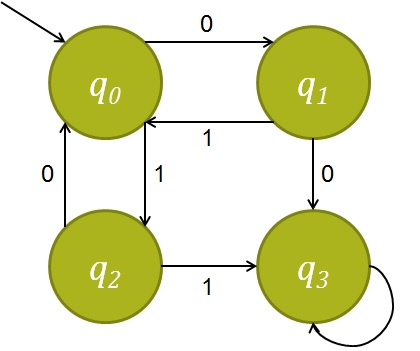
\includegraphics[width=\textwidth,height=\textheight,keepaspectratio]{example}
\end{minipage}
\begin{minipage}[c]{0.7\textwidth}
 \begin{Verbatim}[fontsize=\scriptsize]
node top(x : bool; state: int) returns (  );
var
  bias : int;
  prop1, prop2, prop3, prop4, prop_all : bool;
  bias_max : bool;
let
  bias = 0 -> (if x then 1 else -1) + pre(bias);
  bias_max = false ->
	(bias >= 2 or bias <= -2) or pre(bias_max);
  prop1 = (state = 0 => (bias = 0));
  prop2 = true ->
  	(pre(state = 0) and x) => state = 2;
  prop3 = true ->
  	(pre(state = 0) and not x) => state = 1;
  prop4 = bias_max => state = 3;
  prop_all = prop1 and prop2 and prop3 and prop4;
  --%PROPERTY prop_all;
  --%REALIZABLE x;
tel;
 \end{Verbatim}
\end{minipage}
\caption{Automaton and Requirements for running example}
\label{fg:example}
\end{figure}

% GRIGORY: this sentence is too high-level and too application-specific. I'd start with something more general.
%Considering these requirements, we want an answer to whether this model is
%realizable. We provide the model as an input to \jkind, and observe the results.

Realizability check is needed to identify whether this user-defined model
 has potential conflicts between the requirements.
The model from the example is obviously realizable and has
%, and
%thus can be further examined in terms of synthesizing a representative
%implementation. 
%Using 
the k-inductive proof of length $k = 1$.
The two corresponding $\forall\exists$-formulas ($k=0$ for
the base check, and $k=1$ for the inductive check) are valid, and thus  \aeval
extracts two witnessing Skolem functions
%From this process, we receive two Skolem functions, 
that effectively describe
 assignments to the local variables of the specification, as well as to \texttt{state}.
\grigory{will try to put a snippet of the formula here.} 

The Skolem functions are used to construct the final implementation
following the outline provided in Alg.~\ref{alg:synt}. 
It is 135 lines of code, and due to the space constraints we do not
present it here%
\footnote{The implementation for the
example is available at \url{http://}.}.
The main idea is to redefine each variable in the model 
as an array of size equal to $k$ and
to use the $k$-th element of each array as the corresponding output of the call
to $k$-th Skolem function. After this initialization process, we use an infinite
loop to assign new values to the element corresponding to the last Skolem
function, to cover the inductive step of the original proof. 
\grigory{I'm not sure what you mean by the last sentence. It is long and difficult to parse. If it has some general observation about the algorithm, maybe it makes sense to move to Sect. 2.4?}
One of the
interesting features that come from using Lustre in conjunction with a
k-inductive proof is that we can possibly have properties in the model that
refer to up to $k-1$ values of each variable in the past, and as such an update
process occurs in between each iteration of the infinite loop, to ensure that we
only keep the $k$ latest values of each array.
